\section{Metodologia}
    \begin{frame}[fragile]{Inferência Indutiva}
        \begin{figure}[H]
            \begin{center}
                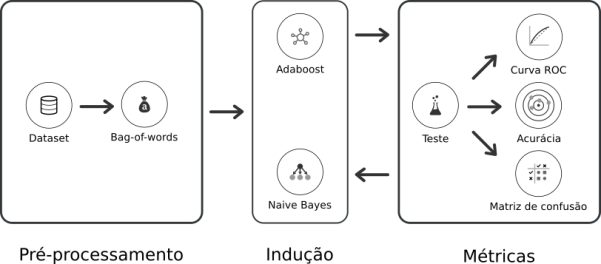
\includegraphics[scale=0.50]{images/inferencia_indutiva.png}
            \end{center}
        \end{figure}
        
        O \textit{dataset} é submetido a técnica \textit{bag-of-words} no 
        pré-processamento, a estrutura de atributo-valor derivada é 
        utilizada no treinamento dos classificadores, por fim, os 
        classificadores são avaliados por métricas de desempenho.
    \end{frame}